\documentclass[a4paper]{article}
\usepackage{geometry}
\usepackage{multicol}
\usepackage{minted}
\usepackage{amsmath, dsfont, mathtools, amssymb}
\usepackage{fontspec}
\usepackage{xcolor}
\usepackage{wrapfig}
\usepackage{graphicx}
\usepackage{enumitem}
\usepackage{wrapfig} 
\usepackage{color,soul}
\usepackage{multirow}
\usepackage{soul}
\usepackage{etoolbox}

\pagestyle{empty}
\geometry{top=0.5cm, bottom=0.5cm, left=0.5cm, right=0.5cm} 

\setlength{\columnsep}{1pt} % Remove space between columns
\setlength{\tabcolsep}{2pt} 


% Redefine section commands to use less space
\makeatletter
\preto{\@verbatim}{\topsep=0pt \partopsep=0pt }
\renewcommand{\section}{\@startsection{section}{1}{0mm}%
                                {-1ex plus -.5ex minus -.2ex}%
                                {0.5ex plus .2ex}%x
                                {\normalfont\normalsize\bfseries}}
% \renewcommand{\subsection}{\@startsection{subsection}{2}{0mm}%
%                                 {-1explus -.5ex minus -.2ex}%
%                                 {0.5ex plus .2ex}%
%                                 {\normalfont\normalsize\bfseries}}
% \renewcommand{\subsubsection}{\@startsection{subsubsection}{3}{0mm}%
%                                 {-1ex plus -.5ex minus -.2ex}%
%                                 {1ex plus .2ex}%
%                                 {\normalfont\small\bfseries}}
\makeatother

% Don't print section numbers
\setcounter{secnumdepth}{0}
\setlength{\parindent}{0em}
\setlength{\parskip}{0.2em}
\setlist[enumerate]{noitemsep, topsep=0pt, leftmargin=*}
\setlist[itemize]{noitemsep, topsep=0pt, leftmargin=*}
\newcommand{\mathcolorbox}[2]{\colorbox{#1}{$\displaystyle #2$}}


\begin{document}

\tiny

\begin{multicols*}{2}
  \section{Evolution of computers}

  Milestones: Vacuum tubes $\to$ Transistors $\to$ Integrated circuits $\to$ Very Large Scale Integration IC (VLSI); \textbf{Moore's Law}: No. Transistors doubles every two years;
  \textbf{Cycle per second} $f$ (Hz); \textbf{Avg cycle per inst} $=\frac{\sum_i CPI_i \times I_i}{\sum_i I_i}$ for each inst $i$ count $I_i$; \textbf{Processor time} $T=\frac{I_c\times CPI}{f}$; Inst per sec $IPS=\frac{f}{CPI}$; MFLOPS: Million float point operations per sec

  \section{Digital logic}

  \begin{tabular}{|c|c|c|c|c|c|c|c|c|}
    \hline
    A & B & NOT                                         & AND                                         & OR                                         & XOR                                         & NAND                                         & NOR                                         & XNOR                                         \\ \hline
      &   & $\overline{A}$                              & $AB$                                        & $A+B$                                      & $A \oplus B$                                & $\overline{AB}$                              & $\overline{A+B}$                            & $\overline{A \oplus B}$                      \\ \hline
    0 & 0 & 1                                           & 0                                           & 0                                          & 0                                           & 1                                            & 1                                           & 1                                            \\ \hline
    0 & 1 & 1                                           & 0                                           & 1                                          & 1                                           & 1                                            & 0                                           & 0                                            \\ \hline
    1 & 0 & 0                                           & 0                                           & 1                                          & 1                                           & 1                                            & 0                                           & 0                                            \\ \hline
    1 & 1 & 0                                           & 1                                           & 1                                          & 0                                           & 0                                            & 0                                           & 1                                            \\ \hline
      &   & 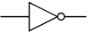
\includegraphics[width=1cm]{./gate-not.png} & 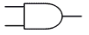
\includegraphics[width=1cm]{./gate-and.png} & 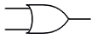
\includegraphics[width=1cm]{./gate-or.png} & 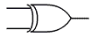
\includegraphics[width=1cm]{./gate-xor.png} & 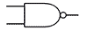
\includegraphics[width=1cm]{./gate-nand.png} & 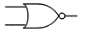
\includegraphics[width=1cm]{./gate-nor.png} & 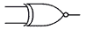
\includegraphics[width=1cm]{./gate-xnor.png} \\ \hline
  \end{tabular}

  \textbf{Sum of product} if mostly 1s, else \textbf{Product of sum};

  \section{Number representation}

  Conver to radix-10: $\sum^{n-1}_{i=0} d_i \times b^i$; Radix-10 to binary: repeatedly divide by 2 and record remainder, fractional part repeatedly multiple by 2 and record integer part

  \textbf{Sign representation} n bits; \textbf{Excess K} $f(b) = b - K$, range $[-K, 2^n - 1 -K]$; top half pos, bottom part neg; \textbf{One's complement}: $f(b) = b \geq 0 ? b : (2^n-1)-b$, range $[-2^{n-1}+1, 2^{n-1}-1]$; \textbf{Two's complement}: $f(b) = b \geq 0 ? b : (2^n-1)-b+1$, range $[-2^{n-1}, 2^{n-1}-1]$, only one that can sum numbers of diff. signs w/o special cases;

  \hl{\textbf{Floating point}} $f$ significand, $e$ exponent, $b$ bias; $\mathrm{sign}\cdot(1.f)\cdot2^{e-b}$; sign,e,f (1,x,l-x-1 bits); sign bit: $+\text{ve} \implies 0$, $-\text{ve} \implies 1$, add trailing zeros $f$ to fill available; range of $e$ is $1\rightarrow254$ for Binary32. $0$ and $255$ are \textbf{reserved for special cases};

  For a given format with $E.bits$ exponent bits, $F.bits$ significand bits and $s=\text{have special case for 0 and } 2^e-1 ? 1 : 0$; \textbf{Range} $\in \pm[2^{s-b},(2-2^{-F.bits})\cdot2^{2^{E.bits-1}-2^{E.bits}-s}]$; Represented numbers are \textbf{unevenly spaced} as spacing depends on exponent, which scales \textit{logarithmically}; \textbf{Spacing grows} as we go further from 0 as scaling factor of $2^{e-(2^{E.bits-1}-1)}$; \hl{\textbf{Precision}}: range $\uparrow$ precision $\downarrow$ (for a set number of bits). Exponent bits is proportional to range, while significand bits is proportional to precision.

  \colorbox{lightgray}{\parbox{.45\textwidth}{\underline{\textit{Converting 13.375 to IEEE Binary32}}: $13.375 \equiv 1101.001_2 \to$ Sign bit: $0$ (pos); expo: normalized $+1.101001_2 \times 2^3$; $f=101001_2$; add trailing zeros: \texttt{10100100000000000000000}; $e=3+b=130\equiv$ \texttt{10000010}; Sol \texttt{0100 0001 0101 0110 0000 0000 0000 0000}}}

  \colorbox{lightgray}{\parbox{.45\textwidth}{\underline{\textit{Converting Binary32 to decimal}} $C0F210000_{16}$: sign \texttt{1}, expo \texttt{10000010}, significand \texttt{11100100000000000000000}; sign bit: $1$ (neg); expo: $10000010_2=130\to 130-127=3$; significand: remove training 0s and add leading "1": $1.111001_2=1.890625_{10}$; value: $-1.890625 \times 2^2 = -7.5625$;}}


  Multiply two's complement: \textbf{shift-and-add}; Add/sub \hl{\textbf{Overflow rule}}: same sign operation, result is different sign

  \colorbox{lightgray}{\parbox{.45\textwidth}{\underline{\textit{Add 1.5 + 2.25}} align expo: $1.1_2 \times 2^0 + 10.01_2 \times 2^0$ Add numbers $10.01_2 + 1.1_2 = 11.11_2$ Normalize $1.111_2 \times 2^1$ Result $1.111_2 \times 2^1 = 3.75$}}

  \colorbox{lightgray}{\parbox{.45\textwidth}{\underline{\textit{Multiply 1.5 * 2.25}} align expo: $1.1_2 \times 2^0 \times 1.001_2 \times 2^1$ Add expo: $0+1=1$ Multiply numbers $1.1_2 \times 1.001_2 = 1.1011_2$ Normalize $11.011_2 \times 2^1$ Normalize $1.1011_2 \times 2^1$ Result $1.1011_2 \times 2^1 = 3.375$}}

  \colorbox{lightgray}{\parbox{.45\textwidth}{\underline{\textit{Multiply IEEE numbers}} $3fc00000_{16} \times 40100000_{16}$: $3fc00000_{16} =$ \texttt{0 01111111 10000000000000000000000}, $40100000_{16} =$ \texttt{0 10000000 00100000000000000000000}; Add exponents and subtract bias: $01111111_2 + 10000000_2 - 01111111_2 \equiv 127 + 128 - 127 = 10000000_2$; Extract numbers by removing trailing zeros and multiply: $1.1_2 \times 1.001_2 = 1.1011_2$; Normalize: $1.1011_2 \times 2^{10000000_2 - 01111111_2}$; Result: \texttt{0 10000000 10110000000000000000000} $=3.375$}}

  \section{Instructions}

  \textbf{PC (Program Counter)}: Holds the address of the next inst to fetch;
  \textbf{MAR (Memory Address Register)}: Holds the memory address for the current read/write operation;
  \textbf{MBR (Memory Buffer Register)}: Temporarily holds data being read from or written to memory;
  \textbf{MDR (Memory Data Register)}: temp data being transferred to or from memory;
  \textbf{IR (Inst Register)}: Holds the current inst being decoded/executed.;
  \textbf{ACC (Accumulator)}: intermediate arithmetic and logic operation results.

  \textbf{Von Neumann archit.}: data \& inst stored in single w/r memo, contents addressable by location, execution seuqential;

  \hl{\textbf{Addressable memory space}}: total amount of memory, determined by \textbf{largest register} width used for memo locations ($2^n$ for n-bit register).

  \textbf{Type of ops.} data transfe, arithmetric, logical, control flow, I/O, data conversion; \textbf{arithmetric} treat operands as numbers, consider sign; \textbf{logical} treat operands as bit patterns;

  \begin{minipage}{.26\textwidth}
    \begin{tabular}{|l|l|l|}
      \hline
      \textbf{Mne}         & \textbf{Assembled}             & \textbf{Assembly Syntax} \\
      \hline
      \texttt{ADD}         & \texttt{00\#\#\#\#\#\#}        & \texttt{src1, src2, dst} \\
      \texttt{SUB}         & \texttt{01\#\#\#\#\#\#}        & \texttt{src1, src2, dst} \\
      \texttt{AND}         & \texttt{02\#\#\#\#\#\#}        & \texttt{src1, src2, dst} \\
      \texttt{OR}          & \texttt{03\#\#\#\#\#\#}        & \texttt{src1, src2, dst} \\
      \texttt{NOT}         & \texttt{04\#\#00\#\#}          & \texttt{src1, dst}       \\
      \texttt{MOV}         & \texttt{05\#\#00\#\#}          & \texttt{src1, dst}       \\
      \texttt{LD}          & \texttt{0600ff\#\# 000000\$\$} & \texttt{adr, dst}        \\
      \texttt{ST}          & \texttt{07\#\#ff00 000000\$\$} & \texttt{src1, adr}       \\
      \texttt{BR} (branch) & \texttt{0800ff00 000000\$\$}   & \texttt{label}           \\
      \texttt{BZ} (0)      & \texttt{0801ff00 000000\$\$}   & \texttt{label}           \\
      \texttt{BNZ} (not 0) & \texttt{0802ff00 000000\$\$}   & \texttt{label}           \\
      \texttt{HALT}        & \texttt{09000000}              & -                        \\
      \texttt{PUSH}        & \texttt{0A\#\#0000}            & \texttt{r}               \\
      \texttt{POP}         & \texttt{0B0000\#\#}            & \texttt{r}               \\
      \texttt{CALL}        & \texttt{0C00ff00 000000\$\$}   & \texttt{label}           \\
      \texttt{RET}         & \texttt{0D000000}              & -                        \\
      \hline
    \end{tabular}
  \end{minipage}
  \begin{minipage}{1\textwidth}
    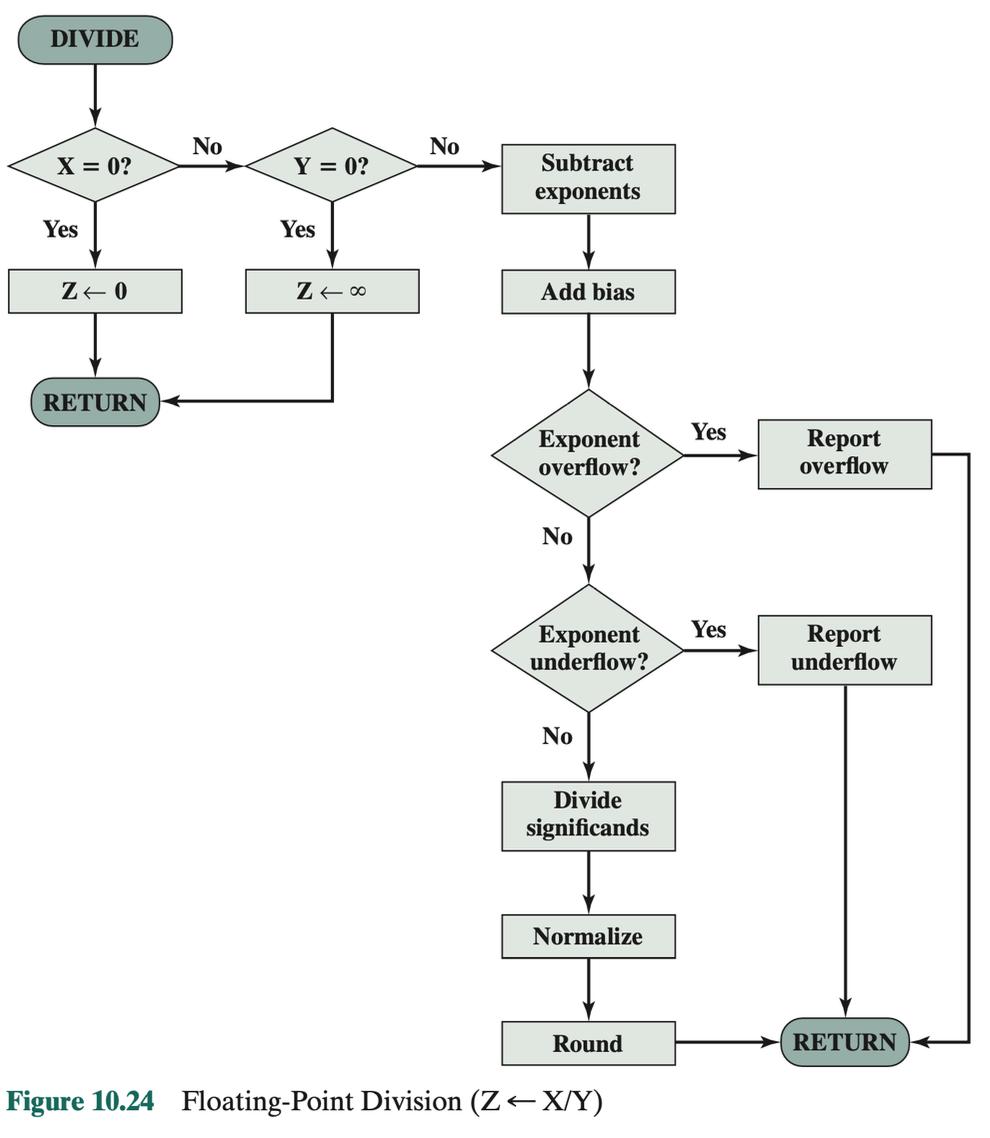
\includegraphics[width=0.18\textwidth]{./fp-division-flow.png}
  \end{minipage}

  \begin{tabular}{|p{1.4cm}|p{1cm}|p{2cm}|p{2cm}|p{2cm}|}
    \hline
    \textbf{Mode}     & \textbf{Notation}                          & \textbf{Explanation}                                           & \textbf{Advantages}     & \textbf{Disadvantages}     \\ \hline
    Immediate         & \texttt{MOV \#5, }                         & Value specified directly                                       & No memory reference     & Limited operand magnitude  \\ \hline
    Direct            & \texttt{MOV 10, }                          & Value in address \texttt{10}                                   & Large operand magnitude & Limited address space      \\ \hline
    Indirect          & \texttt{MOV (10), }                        & Value in address specified in value in address \texttt{10}     & Large address space     & Multiple memory references \\ \hline
    Register          & \texttt{MOV R, }                           & Value of R                                                     & No memory reference     & Limited address space      \\ \hline
    Register Indirect & \texttt{MOV (R), }                         & Value in address specified in value of R                       & Large address space     & Extra memory reference     \\ \hline
    Displacement      & \texttt{MOV 2(R)}                          & Value in \textit{address specified in value of R offset by 2}  & Flexibility             & Complexity                 \\ \hline
    Stack             & \texttt{PUSH R1, <> }, \texttt{POP <>, R1} & \texttt{<>} is the implicit return address stored on the stack & No memory reference     & Limited applicability      \\ \hline
  \end{tabular}

  \hl{\textbf{Techniques}}; \textbf{Set memo location value} \texttt{ST 0b00000000, P1}; \textbf{Read bits of register} \texttt{AND R1, 0b00001111, R1 -> CMP R1, 0b00001010 -> BNE loop} (read last 4 bits if \texttt{1010}, if not then branch to loop); \textbf{Use array at memo location} \texttt{LD LINE, R0 -> LD (R0), R3 -> INC R0} (load first element, get value, next value)

  \textbf{Procedure/Function call/return}: A special type of branch inst where we need to store addr of next inst to be executed (return addr), so that on function return, the program can continue exection at the right place. Nested call requires the return addr to be stored in some dynamic data structure (Stack), return addr are retrieved in LIFO fashion (last function call, first return). Hence, we will store return addr in system stack.

  AC accumulator, T stack; \textbf{Operands}: \textbf{(3)} \texttt{OP A,B,C: A <- B OP C} \textbf{(2)} \texttt{OP A,B: A <- A OP B} \textbf{(1)} \texttt{OP A: AC <- AC OP A} \textbf{(0)} \texttt{OP: T <- (T-1) OP T};

  \textbf{Data types (1)} Numeric (integer, floating point) and \textbf{(2)} Non-numeric(character, binary data). Their lengths are typically 8, 16, 32, or 64 bits.

  \textbf{.data}: tell assembler add all subsequent data to the data section; \textbf{.text}: tell assembler add subsequent code to the text section (i.e. program section); \textbf{.global NAME}: Makes name external to other files, for multiple files in program; \textbf{.space <EXPRESSION>}: Reserves spaces, amount specified by the value of expression in bytes, assembler fills the space with zeros; \textbf{.word exp1 [,exp2]…}: Put the values in successive memory locations.

  \section{Execution cycle}

  \textbf{FDE}: Fetch inst $\to$ Decode inst $\to$ Calculate operand addr $\to$ Fetch operands $\to$ Execute inst $\to$ Write oerand; Many don't need CO, \texttt{LD/ST} don't need EI;

  \textbf{Interruptions} improve eff., I/O need immediate attention, or data may be lost; When interruption is required, I/O device sends a signal to the CPU; \textbf{Timing}: Interrupt signals are checked at the end of one complete instruction cycle, minimising the registers that need to be
  saved/restored. \textbf{Saved information to stack}: Flag register (rmb ALU state), PC (rmb addr next inst), modified register files, current inst. address (rmb where interruption);
  Others not saved as they are only meaningful during the current instruction cycle.

  \section{Memory hierarchy}

  \textbf{Hierarchy}: Registers (inst), On-chip cache (inside cpu), Cache (motherboard), Main (RAM), Secondary storage (disk); left to right: Capacity $\downarrow$,  Cost $\downarrow$,  Access time $\uparrow$,  Access frequency $\uparrow$

  Access: \textbf{(1)} Sequential Access(from front);\textbf{(2)} Random Access; \textbf{(3)} Associative(content-addressable)

  \textbf{Big Endian}: Left to right (abcd); \textbf{Little Endian}: Right to left (dcba) for data[0] = a…

  \textbf{Error Detection}: Even parity (total “1” is even); Odd parity (total “1” is odd); hamming code;

  \hl{\textbf{Principle of Locality}}: address to be referenced next will be close to the current addr; \textbf{Temporal locality}: If a memory location is accessed, it is likely to be accessed again in the near future; \textbf{Spatial locality}: If a memory location is accessed, it is likely that nearby memory locations will be accessed in the near future; \textbf{Importance to caching} allows the cache to predict and retain useful data

  \begin{tabular}{|l|l|l|l|l|}
    \hline
    \textbf{Memory Type} & \textbf{Category}            & \textbf{Erasure}              & \textbf{Write Mechanism}      & \textbf{Volatility}          \\ \hline
    RAM                  & Read-write                   & Electrically, byte-level      & Electrically                  & Volatile                     \\ \hline
    ROM                  & \multirow{2}{*}{Read-only}   & \multirow{2}{*}{Not possible} & Masks                         & \multirow{5}{*}{Nonvolatile} \\ \cline{1-1} \cline{4-4}
    PROM                 &                              &                               & \multirow{4}{*}{Electrically} &                              \\ \cline{1-3}
    EPROM                & \multirow{3}{*}{Read-mostly} & UV light, chip-level          &                               &                              \\ \cline{1-3}
    EEPROM               &                              & Electrically, byte-level      &                               &                              \\ \cline{1-3}
    Flash                &                              & Electrically, block-level     &                               &                              \\ \hline
  \end{tabular}

  \begin{tabular}{|l|l|l|}
    \hline
    \textbf{Characteristic} & \textbf{Dynamic RAM}                          & \textbf{Static RAM}        \\ \hline
    Storage Technology      & Use transistors to store electric charges.    & Use logic gates (latches). \\ \hline
    Refreshing              & Required (every few ms due to leaking charge) & Not required               \\ \hline
    Speed                   & Slower (delay due to capacitance)             & Faster                     \\ \hline
    Usage                   & Main memory                                   & Cache memory               \\ \hline
    Cost                    & Cheap                                         & Very expensive             \\ \hline
  \end{tabular}



  \section{Cache memory}

  \hl{\textbf{Purpose}}: Reduce memory access latency between CPU and main memory

  \textbf{Replacement algorithms}: \textbf{(1)} LRU: least recently used; \textbf{(2)} FIFO: replace the oldest block; \textbf{(3)} Random: randomly select a block to replace; \textbf{(4)} LFU: least frequently used;

  Formulas: see example solutions

  \textbf{Address mapping}: The cache memory splits the given memory address into 3 parts: $[\text{   Tag    }][\text{   Number    }][\text{   Offset    }]$
  ; Offset is used to identify, from left to right, the index of the word in block.

  \begin{tabular}{|p{1cm}|p{1cm}|p{2cm}|p{2cm}|p{1cm}|p{2cm}|}
    \hline
    \textbf{Mapping} & \textbf{bits of "Number"}  & \textbf{Usage of Number}       & \textbf{Usage of Tag}                               & \textbf{Adv.} & \textbf{Disadv.}                                      \\ \hline
    Direct           & $2^s$ = no. of cache lines & Determines cache line directly & Ensures consistency                                 & Fast          & Multiple memory blocks can map to the same cache line \\ \hline
    Full Asso.       & $s = 0$                    & -                              & Matches across all cache lines \textbf{in parallel} & -             & Heavy processing (parallel)                           \\ \hline
    Set Asso.        & $2^s$ = no. of cache sets  & Determines cache set           & Matches within the set \textbf{in parallel}         & -             & -                                                     \\ \hline
  \end{tabular}

  \textbf{Split Cache}: The cache is divided into instruction cache and data cache. Size for each cache is fixed. No pipeline hazard. The main trend is to use split cache;
  \textbf{Unified Cache}: The cache is used for both instructions and data. Instructions and data are automatically balanced. Has contention problem on parallel and pipeline execution that imposes bottleneck on performance.

  \section{External storage}

  \textbf{Average seek time} $T_\text{seek}$: Time taken to move the read/write head to the desired track; \textbf{Average rotational latency }$T_\text{latency}$: Time required for sector to rotate under the head; \textbf{Data transfer time} $T_\text{transfer}$: Time taken to read or write the data once the head is in position;

  \hl{\textbf{Formulas}}: 1 / rps = 60 / RPM; $T_\text{rotation}$ = $rps^{-1}$; $T_\text{latency} = .5 \times T_\text{rotation}$; $T_\text{sector} = T_\text{rotation}\ /\ n_\text{sectors}$; $T_\text{transfer} = \text{bytes}\ /\ \text{bytes per track} \times rps^{-1}$; Time to access $n$ \textbf{consecutive} sectors ignoring transfer speed: $T_\text{seek} + T_\text{latency} + n \times T_\text{sector}$; Time to access $n$ \textbf{non-consecutive} sectors ignoring transfer speed: $(T_\text{seek} + T_\text{latency} + T_\text{sector}) \times n$

  \hl{\textbf{Raid 0}} (Usable \texttt{N}, Failure \texttt{F=0}), adv: simple design, easy to implement, disadv: easy lost data;

  \textbf{Raid 1} (\texttt{N/2} \texttt{F=N/2}), adv: no rebuild is need in case fail, disadv: inefficient;

  \textbf{Raid 2} redundancy (by hamming code), adv: high data transfer rates, disadv: expensive;

  \textbf{Raid 3} Bit interleaved parity (extra HDDs contains parity bit of all other HDDs); adv: high read/write data transfer rate, disadv: complex design for controller;

  \textbf{Raid 5} (\texttt{N-1} \texttt{F=2}) 1 extra HDD needed (parity strip used for error correction), adv: highest data transaction rate, disadv: complex controller design and difficult to rebuild in the event of a disk failure;

  \textbf{Raid 6} (\texttt{N-2} \texttt{F=2}) 2 extra HDDs needed (use two parity strips, calculated using different methods), adv: extremely high data fault tolerance and can sustain multi. simultaneous drive failures, disadv: more complex controller design.

  \textbf{SSD (Solid state Drives)} semiconductor storage, based on flash memory (non volatile), has a limited number of write cycles. Advantages over HDD: High-performance IO Operations, Durability as less susceptible to physical shock and vibration, Longer Lifespan as no mechanical wear, Lower Power consumption as no moving parts, Quieter.

  \section{IO}
  \hl{\textbf{Requirement on IO modules}}: \textbf{Control and Timing} – \textbf{Asynchronous timing}; \textbf{Processor/ Device Communication} – command decoding; \textbf{Data buffering}: store the data in buffer, so that transaction can be more efficient; \textbf{Error detection and correction}.

  \hl{Types}; \textbf{Programmed IO} (no interrupt, high CPU involvement): executes a program that gives it direct control of the IO operation. IO waits for the device to finish its IO operation, wasting CPU time.

  \textbf{Interrupt-driven IO} (use interrupt, medium CPU involvement): alleviate the problem of programmed IO, processor issue an IO command, then continue to execute inst from other process, when IO finish, IO module \textbf{Interrupts} the CPU. The CPU will then suspend the current program, execute remaining IO operations, then return to the suspended program. Processor need to remember current position (done by putting \textbf{PC} and \textbf{Processor Status Word (PSW)} to stack).

  \hl{\textbf{DMA}} (use interrupt, low CPU involvement): uses an intelligent device controller, so as to minimize CPU intervention. IO processor will directly write to the memory; IO processor will \textbf{steal cycles} from the CPU by issuing a signal to tell the CPU to disconnect itself from the bus, and IO device to control memory bus. During this period, the CPU will see an \textbf{elongated clock}, and the CPU will wait for the end of the clock cycle to perform its next action. IO processor reads/writes the memory for one cycle. When IO processor finishes with the current word, removes signal $\to$ CPU continues its normal operation.

  \section{OS support}

  \hl{\textbf{Services provided by OS}}: \textbf{(1) Program creation}: in the form of utility programs that are not actually part of the OS, but are accessible through the OS, e.g. Editor; \textbf{(2)Program execution}: to execute a program, system need to read the program from the HHD to main memory, prepare resources, such as process table...; \textbf{(3) I/O access}: the OS provides a uniform I/O interface to the programs, such as open(), read(), write(), while the detail is left to the OS via the device driver, also prevent user from holding device indefinitely. File system management: how files and directory are created, modified, etc is hidden from the user, file protections, sharing is managed by OS; \textbf{(4) System access}: control access to the system and to specific system resources, protect these resources/data from unauthorized users, e.g. Memory protection: segmentation fault when try to access memory that you are not authorized to.; \textbf{(5) Error detection and response}: report error to programs, and their remedial action; \textbf{(6) Accounting}: collect usage statistics for various resources and monitor performance parameters such as response time, page fault rate...etc

  \textbf{Protection Scheme}: CPU will execute in different mode to facilitate protection; User and kernel mode, (some may have 4 modes). Some resources (such as I/O devices) or actions (some special insts) can only be run in kernel mode, so users will not have access to them. OS is supposed to be well-tested, while bug exist in user programs…, Only OS (in kernel mode) will have the rights; \textbf{Mechanism}: System has to change from user mode to kernel mode to run/use protected resource, OS function are usually accessed via special entry points (sys call)

  \textbf{Multitasking and time sharing system}: CPU idle when IO is performed, to full utilize CPU, CPU shared among process, each process is allocated a time slice, when process uses up it time slice, stop execution, next process executed, can not proceed also stop. \textbf{Process Scheduling}: system maintain a queue of processes base on process priority

  \hl{\textbf{Virtual Memory}}: Memory is limited, especially in a machine with a multitasking OS; \textbf{Logical addressing space}: addressing space as seen by user programs; it is logical, in contrast to \textbf{Physical addressing space}: addresses that are used to actually access the memory. Similar to Cache, it is based on the \textbf{Principle of Locality}, and we use \textbf{Address Mapping} to map logical addresses (of programs) to physical addresses (of memory). Mapping is done by the \textbf{Memory Management Unit (MMU)}; \textbf{vram} is transparent to the user;

  \textbf{Paging}: Logical addressing space: addressing space of your program, e.g., 32-bit address is used, then addressing space is from 0 to 4GB; Physical addressing space: the actual addresses to the physical memory, which can be smaller, e.g., 1GB only. Both addressing spaces are divided into \textbf{Pages} (blocks) of fixed size, say, 4Kbyte pages. Each process will have its own logical addressing space; all programs can start at address 0, if desired; they will be mapped to different places in the physical addressing space.

  \hl{\textbf{Security}}: Each process will need to keep track of a \textbf{Page Table}, which provides information on how to perform memory mapping. Each \textbf{PTE (Page Table Entry)} contains information such as if the page is in memory or not (\textbf{Valid bit, V}); \textbf{Protection information, P}, usually more than 1 bit, indicates the protection mode, such as r/w and kernel/user access; if the page has been changed (\textbf{Dirty bit, D}) to prevent unnecessary write-back when the page has not been changed. \textbf{Page Table} is cached in the \textbf{Translation Lookaside Buffer (TLB)}.

  \textbf{Address Mapping}: MMU not only performs address translation but also protection checking, such as segmentation fault errors; if the page is not in main memory $\to$ \textbf{Page Fault}. The OS will take over, fetch the required page from the hard disk, put it in memory, and restart (HDD IO is slow).

  \textbf{Demand Paging}: When the program starts, nothing is in memory; only bring in pages on demand. \textbf{Adv}: fast response, no need to bring in the entire program for it to start; \textbf{Disadv}: a lot of page faults until a stable working set of the program has been brought into memory. Use \textbf{Prepaging} to bring in a number of pages at the beginning to minimize this.


  \textbf{Address Translation}: Extract the logical page number (MSn-B); find the corresponding PTE and see if the page is in physical memory; \textbf{Yes}: get the physical frame number and append the offset; \textbf{No}: generate a page fault.

  \textbf{Page Fault Handling}: Find the page from HDD; find a free page in physical memory; if none, find one to replace; if the page is dirty, write back to HDD; invalidate the PTE of that page; write the page to that physical page; modify the PTE of the new page to contain correct info.

  \textbf{Page Replacement}: \textbf{FIFO}; \textbf{LRU}; \textbf{Write Strategy}: \textbf{Write back} (common); \textbf{Write through}.

  \textbf{Combining Cache and Virtual Memory}: Perform address translation via \textbf{TLB}, the cache of the page table; if PTE is not in TLB, then use the page table and put the corresponding entry into TLB (only valid pages will be in TLB); obtain the physical address; use this physical address to access cache memory; handle cache misses.

  \section{Processor organization and RISC}

  CPU Execute inst via \hl{\textbf{two operations}}: \textbf{(1)} transfer data via system bus \textbf{(2)} Perform data transformation via ALU.

  % Data are stored in register inside CPU, operation controlled by “Control Signal” (flags) Registers: 2type: user-visible registers, GPR, index registers..; Hidden registers, PC, IR... 

  \textbf{Control Signals}: tell CPU what to do by setting different flags, i.e which bus is used. Signals generated by: \textbf{Hardwired Control} – logic gates, write down the truth table and use logic gates, faster but design is complicated; \textbf{Microprogrammed Control} – control signals are stored in memory(microcodes), entire truth table is stored in mrm, and inputs are the addresses of memory, control store inside cpu, memory access is still slower, easy design Inst Execution Cycle: 3 stages, FI, DI, Inst Execution (CO, FO, EI, WO)

  \textbf{Pipelining} inc. the throughput of the CPU by processing different stages of different insts simultaneously, by having different hardware used for each stage, in one clock cycle; \hl{\textbf{Ideal throughput} 1 CPI}; \textbf{Modern processors} don't have memory operands, so no CO stage.

  \textbf{Resource hazard} When two inst require the same hardware at the same clock cycle; Solutions: Dedicated hardware; Separate cache;

  \hl{\textbf{Data hazard}} Read after write (RAW) when I1 writes to register and I2 reads from it, occur if read before write; Solutions: re-arrange inst., but depends on optimization, or data forwrading; WAR and WAW data hazards possible in parallel systems

  \textbf{Control hazards} When we don't know where to continue until branch inst is executed. The \texttt{FI} stage of next inst cannot start until branch resolved; A branch or jump inst.  can cause the pipeline to stop and be \hl{\textbf{reinitialized}} because it changes the program counter (PC), invalidating instructions already fetched in the pipeline due to a potential change in the instruction flow.

  \textbf{Dynamic Branch Prediction}: need two consecutive wrong predictions to change decision;

  \textbf{Processor performance} Execution Time = Inst Cout $\times CPI \times$ Clock cycle time; Clock cycle time = 1 / Clock rate; Ways to \textbf{improve performance} Simplify inst set and use hardwired logic (Clock rate $\Uparrow$ Inst Count $\uparrow$), extensive pipelining ($CPI \Downarrow$)

  \textbf{RISC}: All inst are register-register type except LD ST; Fixed length and simple, fixed format insts; Relatively few operations and address modes; use of hardwired rather than microprogrammed control; Use of inst pipelining;

  \textbf{Large Register File}: register as cache, compiler mapping – \textbf{Register allocation} (important)

  \textbf{Register Windows}: use portion of register file for parameter passing. Acts as a circular list

  \section{[SOL] Number representation}

  "Convert $0.4$ to 8-bit binary number": \texttt{.4 * 2 = .8 < 0}, \texttt{.8 * 2 = 1.6 > 1}, \texttt{.6 * 2 = 1.2 > 1}, \texttt{.2 * 2 = .4 < 0}...; \texttt{0.4 = 0.0110011}

  \rule{1\linewidth}{0.4pt}

  8-bit two's complement: \textbf{(1)} 76+64: \texttt{01001100 + 01000000 = 10001100}; \textbf{Overflow} as result is negative;
  \textbf{(2)} (-42) - 40: \texttt{11010110 + 11011000 = 110011110 -> 10011110} \textbf{Carry out} (no overflow) as result is properly negative;

  \rule{1\linewidth}{0.4pt}

  40-bit floating point representation, biased exponent E 11 bits, significand f 28 bits; No special meanings for E = \texttt{11...1} and \texttt{00...0}; $V = (-1)^{S} \times 1.f \times 2^{E - 1023}$

  \rule{1\linewidth}{0.4pt}

  "Prove that the multiplication of an n-bit binary number A and an m-bit binary number B gives a product A $\times$ B of no more than n + m bits."

  Largest possible value of A is $2^n - 1$ and B is $2^m - 1$. So, the largest possible value of A $\times$ B is $(2^n - 1) \times (2^m - 1)$. If n is equal to m, we get a maximum of $2^{n+m} - 1$.

  \textbf{Largest positive number} $(2-2^{-28}) \cdot 2^{1024}$; \textbf{Smallest positive number} $2^{-2^{10}+1} = 2^{-1023}$;

  \section{[SOL] Instructions}

  \begin{minipage}{0.2\textwidth}
    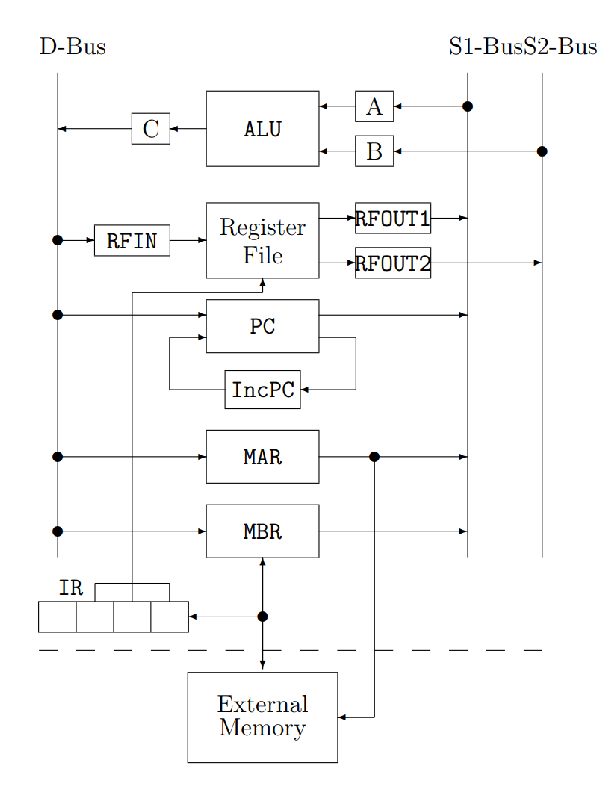
\includegraphics[width=\textwidth]{./ex-cpu.png}
  \end{minipage}
  \begin{minipage}{0.25\textwidth}
    "\ul{Describe the basic operations involved in reading the next inst into IR (inst fetch)}"
    $\star$ Move the value of PC to MAR via S1-bus and D-bus; Perform a memory read, and the data will be written to IR

    "\ul{Show the operations for executing \texttt{ADD R1, R2, R3}}"
    $\star$ Instruction fetch as in previous part; Read the Register File. R1 and R2 will be in RFOUT1 and RFOUT2; move RFOUT1 to A via S1-bus, RFOUT2 to B via S2-bus; Perform ALU Add. Result in C; move C to RFIN via D-bus; Write Register File, writing the value in RFIN to R3

    "\ul{If we reduce to a single CPU bus (instead of three), how is performance affected?}"
    $\star$ With three separate busses, the CPU can read two registers simultaneously and feed them to ALU; Using only one bus, each source register read would happen sequentially, requiring extra cycles to transfer operands before the ALU can operate; Effect: CPU performance decreases (more clock cycles per instruction)
  \end{minipage}

  \rule{1\linewidth}{0.4pt}

  \begin{minipage}{0.2\textwidth}
    Data transfer sequence \texttt{ADD R1, R2, R3}:
    \begin{verbatim}MAR <- PC
PC <- PC + 4  
IR <- mem[MAR] 
CO1: MAR ←− PC
      PC ←− PC+4
      MBR ←− mem[MAR]
      MAR ←− MBR
FO1: MBR ←− mem[MAR]
      ALU.i1 ←− MBR
CO2: MAR ←− PC
      PC ←− PC+4
      MBR ←− mem[MAR]
      MAR ←− MBR
FO2: MBR ←− mem[MAR]
      ALU.i2 ←− MBR
EI:  ALU.output ←− ALU.i1 + ALU.i2
CO3: MAR ←− PC
      PC ←− PC+4
      MBR ←− mem[MAR]
      MAR ←− MBR
WO:  MBR ←− ALU.out
         mem[MAR] ←− MBR
    \end{verbatim}
  \end{minipage}
  \begin{minipage}{0.25\textwidth}
    Custom DIV:
    \begin{verbatim}
# in R10  dividend
# in R11  divisor
# out R12 quotient 
# out R13 remainder 
MYDIV:  SUB R12, R12, R12
        MOV R10, R13
        REP: SUB R13, R11, R13
        BMI END1 # branch if minus
        INC R12
        GOTO REP
END1:
        ADD R13, R11, R13
        RET
        \end{verbatim}
  \end{minipage}

  \rule{1\linewidth}{0.4pt}

  "\textit{System with one-instruction format. How many operands do the \texttt{ADD R1} intruction have, and where are the other operands not specified? }"
  Three: 2 source 1 dest operand; R1 is one of source, others implied at accumulator (previous inst.)

  \rule{1\linewidth}{0.4pt}

  "\textit{What kind(s) of pipeline hazard exist in the instruction"} \texttt{ADD R1, SUB R3}? \textit{Suggest way to re-design instruction so there will be less pipeline hazard.}"
  Data hazard as data dependency between instructions; R1 modifies accumulator and R3 reads from it, if R1 not written back before R3 write, RAW hazard occurs; Solution: redesign format to support explicit source and dest reoperands (or if not change format, add 2-3 insts. between)


  \section{[SOL] Cache memo}

  "Machine: 1024 words of cache memory, Organized as two-way set associative, Cache block size: 128 words, 1 word = 4 bytes, Byte-addressable memory, Address example: \texttt{C912F}$_{16}$ (hex)"

  No. blocks: \texttt{1024 / 128 = 8}; No. sets: \texttt{8 / 2 = 4}; Block size / no. bytes per block: \texttt{128 * 4 = 512};  Set bits: \texttt{log2(4) = 2}; Offset bits: \texttt{log2(512) = 9}; Tag bits: \texttt{20 - (9 + 2) = 9}; (Tag-set-offset)

  \texttt{C912F}$_{16} \to$ $\texttt{1100 1001 0001 0010 1111}_2$;

  Tag: \texttt{110010010}$_2$ = 402; Set: \texttt{00}$_2$ = 0; Offset: \texttt{100101111}$_2$ = 303;

  Cache block containing address's range: \textbf{(1)} lower: set offset to 0 \texttt{C9000}$_{16}$, \textbf{(2)} upper: add block size to lower \texttt{C91FF}$_{16}$;

  \rule{1\linewidth}{0.4pt}

  "Machine: \textbf{w=512 words} of \ul{cache memory (size)}, \textbf{two-way set associative}, \ul{cache block size} of \textbf{s=64 words}, \textbf{LRU} replacement algorithm. Suppose the \ul{cache hit time} is \textbf{th=8ns}, \ul{time to transfer first word} from main memory to cache \textbf{t0=60ns}, \ul{subsequent words} \textbf{t=10ns/word};"

  "Consider the following read pattern (in blocks of 64 words, and block id starts from 0):
  \texttt{A = [1 2 3 4 5 6 8 9 10 5 6 8 4 5 9 10 1 2 3 4 12 16 17 18 16 17 18 16]}
  and assume each block contains an average of \textbf{ar=32 references}.

  \textbf{* Cache miss penalty} \texttt{tp = t0 + t(s-1)};

  \textbf{* Block count count} \texttt{b = w / s};
  \textbf{* Set count} \texttt{n = b / 2};

  \textbf{* Content of cache memory}: First compute $x\%n \forall x \in A$ (the insertion history, remainder is the belonging set). For set \texttt{0}, \texttt{[4 8 4 4 12] -> [4 12]}...;

  \textbf{* Number of cache miss}: For set \texttt{0}, no. misses is size of \texttt{[4 8 12]=3};

  \textbf{* Cache hit rate}: Find no. misses, \texttt{P(hit)=1-[no.misses/(len(A) * ar)]};

  \textbf{* Avg. memo access time} \texttt{AMAT = th + tp * (1-P(hit))};

  \textbf{* Byte addressable address offset, set, tag}: Block size in bytes = \texttt{s * 4 = 256}; Offset bits = \texttt{log2(256) = 8}; Set bits = \texttt{log2(4) = 2}; Tag bits = \texttt{20 - (8 + 2) = 10};

  \textbf{* Instead direct-mapped address offset, set, tag}: Same offset bits; Set bits = \texttt{log2(b)}; Compute new tag bits

  \rule{1\linewidth}{0.4pt}

  "\textit{System with \textbf{two level cache}, L1: cache size \# words, th1=1ns, pHit1=.65, L2: cache size \# words, th2=6ns, pHit2=.95, block size s=128 bytes; System can read 4 32-bit words in parallel; First 4 words t0=60ns / 4 words, t=12ns / 4 words}"

  \textbf{* Cache miss penalty level 2} \texttt{32 / 8bit = 4} byte words $\to$ \texttt{tp = t0 + (s-4*4) * t / 4*4};

  \textbf{* Memo access time} \texttt{MAT1 = th1, MAT2 = th2}

  \textbf{* MAT if data in main mem} \texttt{MATa = th1 + th2 + tp}

  \textbf{* AMAT} \texttt{AMAT = MAT1 * (pHit1) + (1-pHit1) * pHit2 * MAT2 + (1-pHit1) * (1-pHit2) * MATa}

  \rule{1\linewidth}{0.4pt}

  "\textit{Write program to loop over elements of a 2D array that is stored in the system that uses the column-major scheme (memo stores column per column). Program must reduce memo access time assume having cache system, and explain why time can be reduced.}"

  \texttt{for i from 0 to n-1//for j from 0 to n-1//print A[j][i]}; Memo locations addressed sequentially, improves spatial locality (once a memory block fetched into cache, adjacent elements in the same block are already available in the cache). This reduces cache misses and improves performance.

  \section{[SOL] Storage}

  "\textit{Laptop with 4GB mem, 64GB SSD. Light on SSD flashing and running slow. Explan why and how fix.}"
  Low ram, high disk I/O (paging), close not using apps to free ram or add more RAM

  \rule{1\linewidth}{0.4pt}

  "\textit{RAID 5 is employed with six 10 T HDDs. What is the overall storage capacity? what about RAID 1 and RAID 6?}"

  RAID 5 uses $(N-1)$ disks' worth of capacity for data when there are N total disks: $(6-1)\times10T$; RAID 6 uses $(N-2)$ disks' worth of capacity for data (two parity blocks): $(6-2)\times10T$; RAID 1 uses $(N/2)$ disks' worth of capacity for data (mirroring): $(6/2)\times10T$;

  \rule{1\linewidth}{0.4pt}

  "\textit{Improve performance for machine with SSD and HHD}"

  Use SSD to store programs and frequent files, and HDD to store infrequently used static data;


\end{multicols*}
\end{document}

% \colorbox{lightgray}{\parbox{.45\textwidth}{\underline{\textit{...}} }}